\documentclass[11pt]{article}
\usepackage{mathtools,hyperref,booktabs,fullpage, txfonts}
\usepackage[amssymb,cdot]{SIunits}
\usepackage[utopia]{mathdesign}     

\usepackage[table]{xcolor}
\usepackage{xcolor}
\usepackage{soul}
\usepackage{amsmath}
\usepackage{hyperref}
\usepackage{longtable}
\usepackage{fullpage}
 
\definecolor{lightgray}{gray}{0.93}

\pagestyle{empty}
\setlength\parindent{0pt}
\renewcommand{\thefootnote}{\fnsymbol{footnote}}
 
\makeatletter
\renewcommand\section{\@startsection{section}{1}{\z@}%
                                  {-3.5ex \@plus -1ex \@minus -.2ex}%
                                  {2.3ex \@plus.2ex}%
                                  {\normalfont\bfseries}}
\makeatother


\begin{document}

{\large
  \begin{center}
    {\bf ME 701 -- Development of Computer Applications In Mechanical Engineering \\ 
         Homework 2 -- Due 9/13/2017 \\
         Submitted By: John Boyington
    }
  \end{center}
}
 

\section*{Problem 1 -- More in the Command Line}
The commands I used to accomplish the tasks in problem 1: 
\begin{figure}[h]
	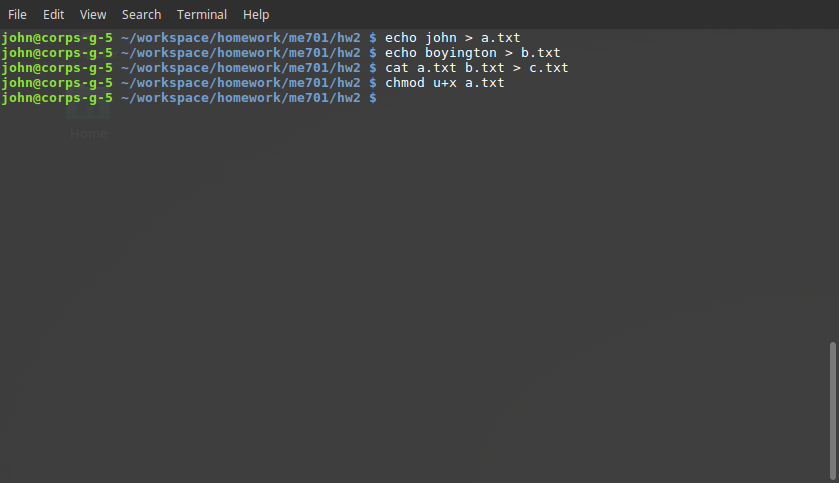
\includegraphics[height=8cm]{me701_hw2_p1_1}
\end{figure}

\section*{Problem 2 -- Simple Shell Scripting}
The scripts that accomplish each task are located in my git repository and named:
\begin{enumerate}
 \item temp.sh 
 \item count.sh
 \item trashTruck.sh
\end{enumerate}
respectively.

\section*{Problem 3 -- Git and Version Control}
To access my files, you can go to my homework repository: \href{https://github.com/johnboyington/homework}{https://github.com/johnboyington/homework}\\
The scripts are located under: /me701/hw2 \\
The kelvin feature was added in commit: c8851d1

\end{document}
